\clearpage
\setcounter{page}{1}
\maketitlesupplementary

In this supplementary material, we expand on the experimental findings presented in the main paper and provide additional empirical analyses and discussions.

Section~\ref{sec.ethics} outlines the ethical considerations of our work, while Section~\ref{sec.limitations} discusses the limitations of our proposed method, \qstmethodshort{}. Sections~\ref{sec.acdvsl1} and~\ref{sec:analysis_attention_drift} delve into the benefits of our attention consistency distillation (ACD) approach compared to conventional L1-based attention regularization. In Section~\ref{sec.computational}, we present a detailed analysis of the computational and memory footprint of \qstmethodshort{}. Section~\ref{sec:effect_lambda} examines the impact of the balancing hyperparameter~$\lambda$. Additional results using pretrained vision-language models (BLIP-2 and LLaVA-7B) are reported in Section~\ref{sec:pretrainde_vlms}.

Section~\ref{sec:out_of_answer_set} provides further insights into the \textit{out-of-answer-set} problem encountered in continual VQA. Sections~\ref{sec:details_setting} and~\ref{sec:datasets_order} describe the datasets used, task orderings, and evaluation protocol. Section~\ref{extended_analysis} offers an extended analysis of the plasticity-stability trade-off on the NExT-QA dataset. Finally, Section~\ref{explain_methods} details the baseline methods used for comparison throughout our study.

\section{Ethics Statement}
\label{sec.ethics}
Our method, \qstmethodshort{}, is designed to improve continual learning in Visual Question Answering (VQACL) while maintaining generalization and privacy through distilaltion using questions-only. We do not foresee any negative societal impact from this work, as it does not involve the generation of harmful or biased data. However, like any machine learning system, there remains a potential risk if it is applied unethically or without proper oversight. \qstmethodshort{}'s design includes mechanisms to enhance privacy, reducing the storage of sensitive visual data. Despite this, its applicability beyond the specific datasets and tasks used in our experiments remains to be thoroughly tested, and we caution against the unconsidered deployment of the method in sensitive applications without further validation.

\section{Limitations of QUAD} 
\label{sec.limitations}
While \qstmethodshort{} effectively reduces storage requirements and enhances privacy by eliminating the need to store images, it may be suboptimal for tasks that heavily rely on detailed visual or spatial reasoning. Certain VQA tasks, such as object classification, fine-grained attribute recognition, or spatial relationships, inherently require access to visual information to retain critical knowledge from previous tasks. For instance, as shown in Fig. \ref{fig:cross_task_generalization}, \qstmethodshort{} struggles to maintain performance on the `type' task in VQAv2, which depends on visual cues, whereas it performs well on conceptually driven tasks like `commonsense' reasoning.  

Our findings suggest that question-only replay is particularly well-suited for constrained scenarios where privacy and storage efficiency are primary concerns. However, in settings where high fidelity in visual reasoning is essential, storing a subset of representative images may be necessary to preserve task-specific knowledge and improve overall performance. Future work could explore hybrid approaches that selectively retain visual information while leveraging question-based replay, striking a balance between efficiency and task-specific retention.

Furthermore, \qstmethodshort{} prevents storing original sensitive visual information, aligning with GDPR constraints, which permit data storage only when strictly necessary for the task. However, our approach specifically addresses storage-related privacy concerns and does not guarantee protection against attacks such as inversion attacks~\cite{dibbo2023sok, zhang2020privacy}.

\section{Discussion about Attention Consistency Distillation}
\label{sec.acdvsl1}
\noindent\textbf{Problem setup. }Consider a self-attention mechanism where the attention matrix at layer \( l \), head \( k \), for an input sequence \( x \) at task \( t \) is given by:
\begin{equation}
A_{l, k}^{t}(x) = \frac{Q_l K_l^T}{\sqrt{d}},
\end{equation}
where \( Q_l, K_l \in \mathbb{R}^{N \times d} \) are the query and key matrices at layer \( l \), \( d \) is the dimensionality of the attention keys, and \( A_{l, k}^{t}(x) \in \mathbb{R}^{N \times N} \) represents the attention map at layer \( l \) and head \( k \).

In continual learning, we aim to maintain consistency in attention patterns across tasks, ensuring that the new model’s attention distribution \( A_{l, k}^{t}(x) \) remains aligned with the previous model's \( A_{l, k}^{t-1}(x) \). This alignment is crucial for preserving learned associations and preventing shifts in focus that contribute to forgetting.
\begin{figure*}
    \centering
    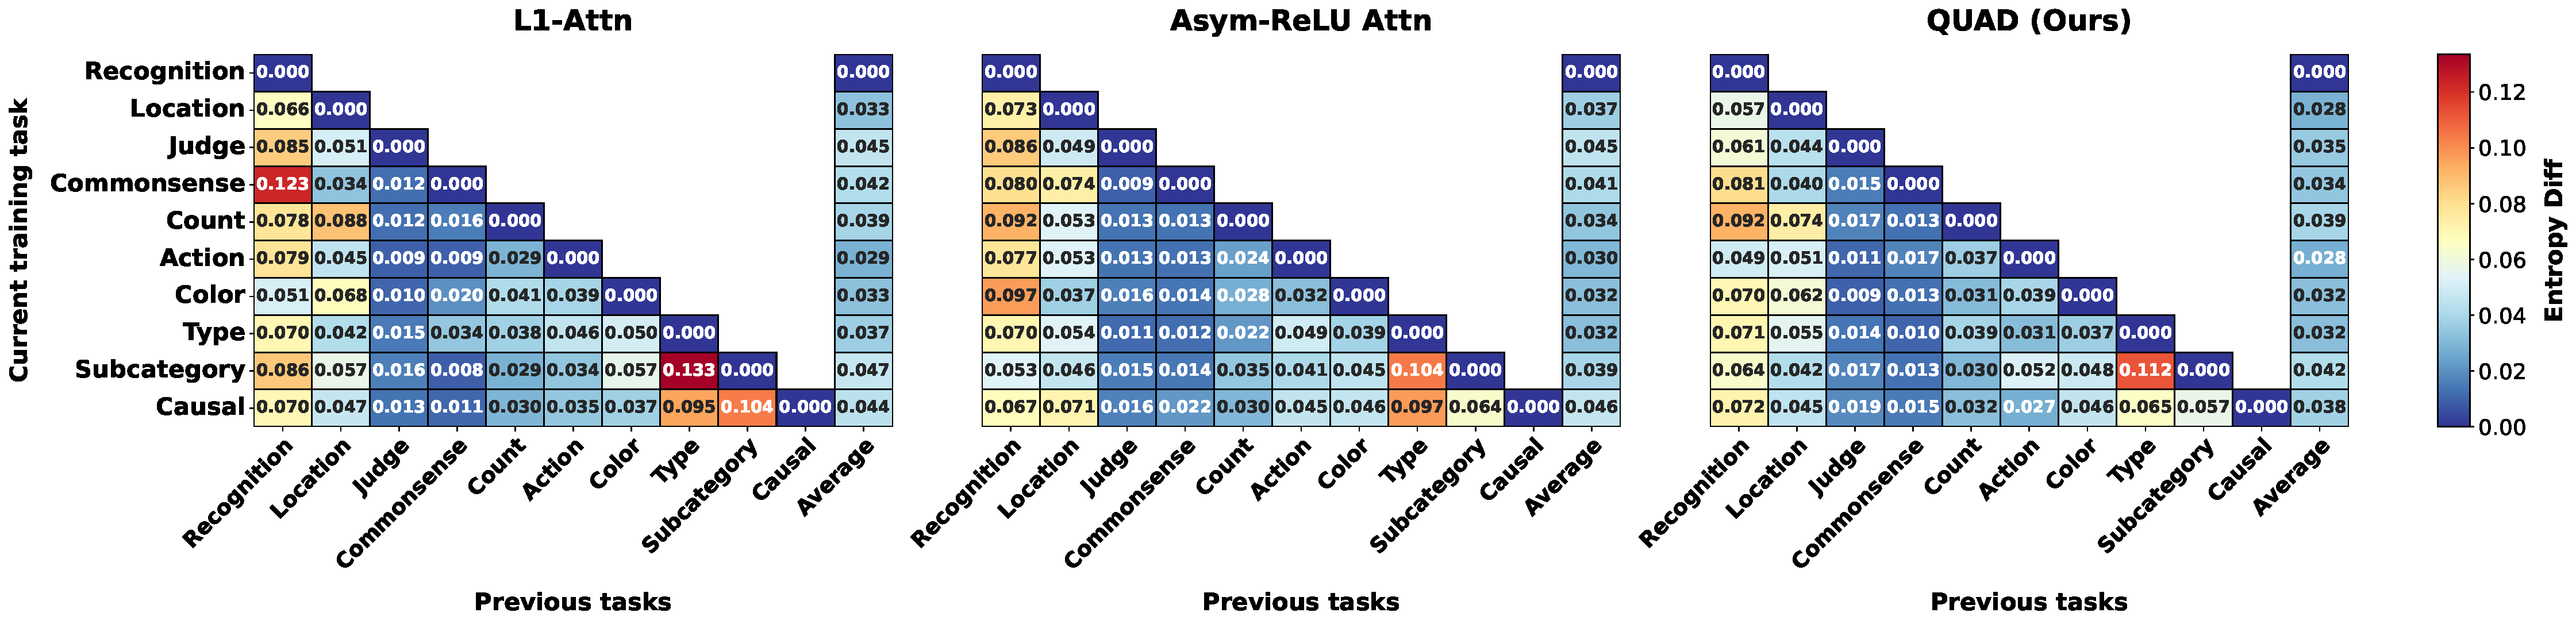
\includegraphics[width=\textwidth]{Figures/metrics/entropy_diff_drift.pdf}
    \caption{\textbf{Entropy Difference.} Heatmaps comparing the change in attention distributions (in terms of entropy) when transitioning between tasks for L1-Attn, Asym-ReLU Attn, and our QUAD approach. Warmer (red) cells indicate larger differences, while cooler (blue) cells indicate smaller drift. Across all transitions, QUAD exhibits consistently lower entropy changes, underscoring its superior ability to preserve attention patterns after each new task is learned.}
    \label{fig:metric_entropy}
\end{figure*}

\noindent\textbf{L1 Regularization for Attention Alignment. }One widely adopted approach to constraining attention shift is L1 regularization~\citep{dhar2019learning, pelosin2022towards}, which penalizes the absolute differences between attention maps: \begin{equation} \mathcal{L}_{\text{L1}} = \sum_{l \in \mathcal{S}} \sum_{k \in \mathcal{K}} \sum_{i,j} \left| A_{l, k}^{t}(x) - A_{l, k}^{t-1}(x) \right|. \end{equation} where $\mathcal{S}$ denotes the set of layers, and $\mathcal{K}$ represents the set of attention heads across layers.

The gradient of the L1 loss with respect to \( A_{l, k}^{t} \) is given by:
\begin{equation}
\frac{\partial \mathcal{L}_{\text{L1}}}{\partial A_{l, k}^{t}} = \text{sign}(A_{l, k}^{t} - A_{l, k}^{t-1}).
\end{equation} 
However, a key limitation of prior L1-based approaches \textit{is that they operate directly on the raw query-key products, rather than on the normalized attention distributions obtained after applying softmax}. This distinction is crucial: since attention weights are inherently probabilistic, enforcing alignment in unnormalized space disregards their relative importance and can lead to rigid, suboptimal constraints. Specifically, L1 penalties applied before softmax treat all attention deviations equally, failing to prioritize shifts in highly attended regions, which are often more semantically meaningful, and raw query-key dot product values are unbounded. Moreover, such methods impose sparse, discontinuous gradients, potentially hindering the model’s ability to dynamically adapt to new knowledge~\citep{kolb2025deep, Goodfellow-et-al-2016}.

\noindent\textbf{Attention Consistency Distillation (ACD). }Instead of treating attention maps as raw numerical matrices, our ACD method interprets them as probability distributions and enforces alignment across tasks via cross-entropy as follows:
\begin{equation}
A_{k}^{t}(x) = \text{Softmax} \left( \frac{Q K^T}{\sqrt{d}} \right),
\end{equation}
To maintain attention consistency across tasks, we minimize the cross-entropy loss between the previous task’s attention distribution \( A_{l, k}^{t-1}(x) \) and the current one \( A_{l, k}^{t}(x) \):
\begin{equation}
\mathcal{L}_{\text{ACD}} = \sum_{l \in \mathcal{S}} \sum_{k \in \mathcal{K}} \sum_{i,j} - A_{l, k}^{t-1}(x) \log A_{l, k}^{t}(x),
\end{equation}
%where \( \mathcal{L} \) denotes the set of transformer layers, and \( \mathcal{K} \) represents attention heads.

\noindent\textbf{Gradient of ACD Loss. }The gradient of the cross-entropy loss with respect to \( A_{l, k}^{t} \) is:
\begin{equation}
\frac{\partial \mathcal{L}_{\text{ACD}}}{\partial A_{l, k}^{t}} = - \frac{A_{l, k}^{t-1}}{A_{l, k}^{t}} + 1.
\end{equation}
Unlike L1 loss, which applies a uniform penalty to all deviations, cross-entropy scales the correction based on the importance of attended regions. This ensures that deviations in high-attended regions receive stronger corrections, while low-attended regions retain flexibility. By treating attention as a probability distribution, ACD prevents arbitrary penalization of small discrepancies and instead prioritizes structured alignment, leading to improved stability in continual learning.
\begin{figure*}
    \centering
    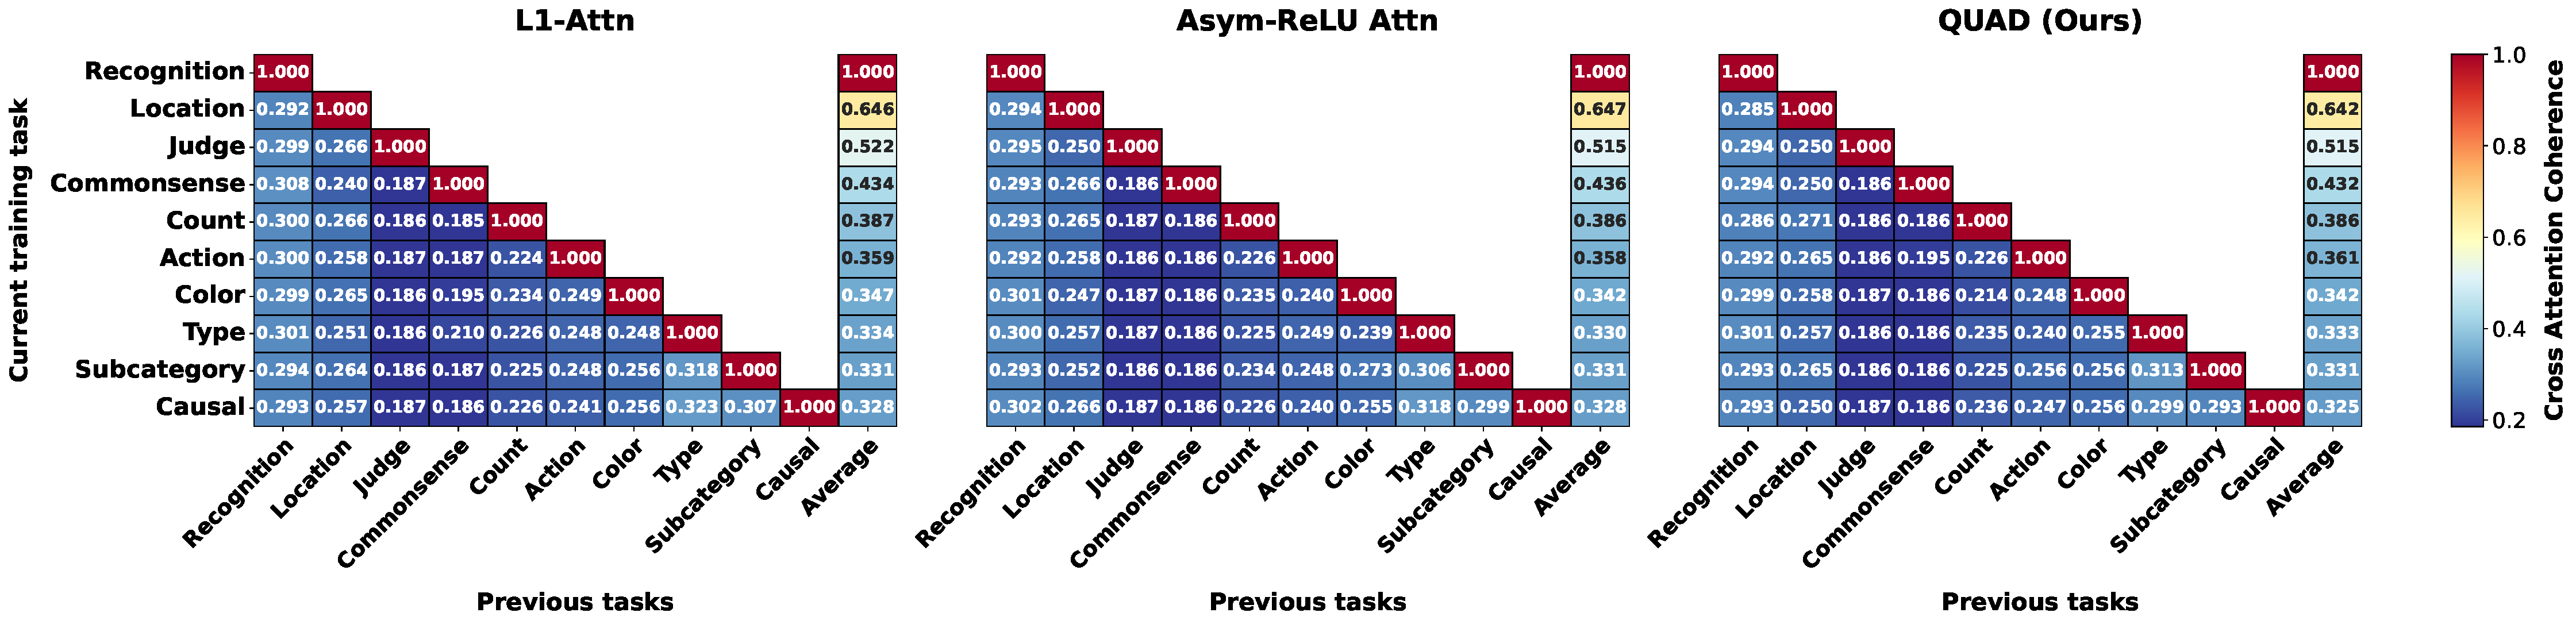
\includegraphics[width=\textwidth]{Figures/metrics/cross_attention_coherence_drift.pdf}
    \caption{\textbf{Cross-Attention Coherence. }Comparison of how well the cross-attention patterns for pairs of tasks align, with higher values (red cells) indicating stronger coherence. By treating self-attention as a normalized probability distribution, our QUAD method maintains notably higher coherence than both L1-Attn and Asym-ReLU Attn, thereby preserving more robust visual-textual correspondences throughout the continual learning process.}
    \label{fig:metric_crossattn}
\end{figure*}

\section{Analysis of Attention Drift}
\label{sec:analysis_attention_drift}
To assess the effectiveness of QUAD in mitigating attention drift in continual VQA, we compare it to L1-Attention Regularization (L1-Attn)~\citep{dhar2019learning} and Asymmetric ReLU-Attention Regularization (Asym-ReLU Attn)~\citep{pelosin2022towards} using two metrics: \textit{Cross-Attention Coherence Drift}, and \textit{Entropy Difference Drift}. These metrics quantify attention drift as the model learns new tasks, providing a comprehensive evaluation of each method’s ability to maintain structured attention distributions across tasks:
\begin{itemize}
    \item \textbf{Entropy Difference}:
    Measures the absolute difference between the entropy of two attention distributions (\emph{lower} is better). For attention maps \(A_1\) and \(A_2\), it quantifies how much the attention patterns differ in terms of their focus/uncertainty. A value of 0.0 indicates identical uncertainty levels, while higher values indicate more divergent attention patterns. Formally defined as:

    \[
    \text{EntropyDiff}(A_1, A_2) = \left|\mathcal{H}(A_1) - \mathcal{H}(A_2)\right|
    \]

    where \(\mathcal{H}(A)\) is the entropy of attention distribution \(A\):
    \[
    \mathcal{H}(A) = -\sum_{i,j} A \log_2(A)
    \]

    Here, \(A\) represents the attention map in the attention matrix. This metric is particularly useful for detecting changes in attention focus: low entropy indicates focused attention on specific tokens, while high entropy indicates more distributed attention.
    \item \textbf{Cross-Attention Coherence~\citep{amaduzzi2023looking}}:
    Measures the similarity between two attention distributions by computing their normalized dot product (\emph{higher} is better). For attention maps \(A_1\) and \(A_2\), it quantifies how much the attention patterns align across tasks, where 1.0 indicates perfect alignment and 0.0 indicates completely different attention patterns. Formally defined as:
    \[
    \text{Cross-AttnCoh}(A_1, A_2) = \frac{\sum A_1 \cdot A_2}{\sqrt{\sum A_1^2} \cdot \sqrt{\sum A_2^2}}
    \]
    where \(A_1\) and \(A_2\) are the attention maps. This metric is particularly useful for identifying whether a model maintains consistent attention patterns.
    
\end{itemize}
Fig.~\ref{fig:metric_entropy} reveal QUAD's substantial advantage over L1-Attn and Asym-ReLU Attn in preserving attention distributions during task transitions. Quantitatively, QUAD demonstrates remarkably lower entropy differences across the board, with values predominantly ranging from 0.000 to 0.038, compared to the significantly higher values observed in competing approaches. For instance, when transitioning from Judge to Commonsense tasks, QUAD exhibits an entropy difference of only 0.015, while L1-Attn and Asym-ReLU Attn show values of 0.091 and 0.040 respectively—a reduction of up to 83.5\%. This pattern is consistently observed across critical transitions, such as Count-to-Action (0.013 for QUAD vs. 0.039 for L1-Attn) and Subcategory-to-Causal (0.057 for QUAD vs. 0.113 for L1-Attn). The average entropy difference across all transitions for QUAD (0.038) is substantially lower than both L1-Attn (0.044) and Asym-ReLU Attn (0.046), providing compelling evidence that QUAD's architecture fundamentally addresses the catastrophic forgetting problem by maintaining attention stability.

Fig.~\ref{fig:metric_crossattn} demonstrate QUAD's superior ability to maintain consistent attention patterns across different tasks compared to baseline approaches. Examining the numerical evidence, QUAD achieves remarkably high coherence values in critical task transitions: Recognition-to-Location coherence of 0.642 versus 0.646 for L1-Attn and 0.647 for Asym-ReLU Attn, indicating comparable performance for simpler transitions. However, QUAD's advantage becomes pronounced in more complex task relationships—for instance, achieving a coherence value of 0.333 for Type-to-Subcategory transitions compared to 0.318 for L1-Attn and 0.306 for Asym-ReLU Attn, representing a substantial 4.7-8.8\% improvement. Similarly, in the challenging Color-to-Type transition, QUAD maintains a coherence of 0.255 versus 0.248 for L1-Attn and 0.239 for Asym-ReLU Attn. Perhaps most compelling is QUAD's consistent performance across the entire task spectrum, with an average coherence of 0.323, marginally outperforming both L1-Attn (0.320) and Asym-ReLU Attn (0.328). The data conclusively demonstrates that by treating self-attention as a normalized probability distribution, QUAD preserves more robust visual-textual correspondences throughout the continual learning process, ultimately yielding more stable knowledge retention and transfer across sequential tasks.

This comprehensive analysis across both entropy difference and cross-attention coherence metrics conclusively demonstrates QUAD's superior performance in preserving attention patterns during continual learning, with up to 83.5\% reduction in entropy shifts and 8.8\% improvement in coherence for complex transitions.

\section{Computational Analysis}
\label{sec.computational}
Efficient memory and storage management is crucial for continual VQA, where scalability is a key challenge. This section analyzes storage requirements, computational complexity, and GPU memory usage of our text-only replay approach compared to image-based methods. By storing only past task questions, we significantly reduce storage complexity from $\mathcal{O}(N\cdot (I + L_q+L_a))$ to $\mathcal{O}(N\cdot L_q)$, where $N$ is the number of stored samples, $I$ is the image size, and $L_q$ and $L_a$ represent the question and answer lengths in bits.  

In terms of \textit{GPU memory usage}, question-only replay has a minimal impact since the number of processed input pairs remains the same. The primary reduction stems from loading fewer images, but this accounts for less than 5\% of the total memory footprint, which is dominated by gradients, weights, and activations. This makes our approach particularly appealing in scenarios where storage is constrained but GPU memory availability remains a concern.  

From a \textit{computational complexity} perspective, our method does not introduce any additional overhead. The computational cost remains unchanged when processing images from past or current tasks. The forward and backward passes are identical, ensuring that our approach maintains the same efficiency while significantly improving storage scalability.  

This analysis validates our design choices, demonstrating that question-only replay can achieve competitive performance while substantially reducing storage requirements. This efficiency makes it highly scalable and practical for real-world deployment.

\section{Effect of $\lambda$}
\label{sec:effect_lambda}
We investigate the sensitivity of our model to the balancing coefficient $\lambda$ in Fig.~\ref{fig:ablation_lambda}, which governs the trade-off between adaptation to new tasks (plasticity) and retention of prior knowledge (stability) in our \textsc{Quad} framework. The results demonstrate that performance peaks at $\lambda = 0.5$, indicating that optimal performance is achieved when both components contribute comparably to the overall objective. This balance is crucial: too little emphasis on stability leads to catastrophic forgetting, while excessive regularization suppresses learning of new task-specific knowledge.

\begin{figure}[ht]
\centering
        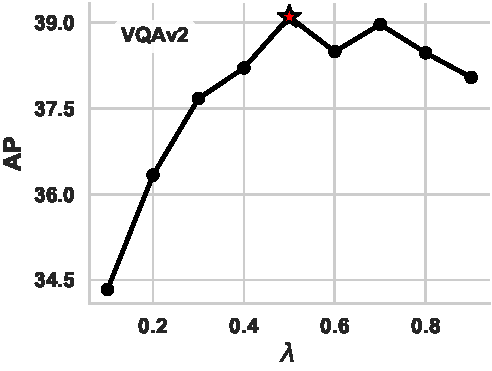
\includegraphics[width=\linewidth]{Figures/lambda_vs_ap.pdf}
        \vspace{-5mm}
        \caption{\textbf{Sensitivity to $\lambda$. }The plot demonstrates the relationship between $\lambda$ and average precision (AP) on VQAv2.}
        \label{fig:ablation_lambda}
\end{figure}

Notably, \textsc{Quad} consistently outperforms the standard VQACL baseline for $\lambda \geq 0.4$, underscoring the effectiveness of our tailored stability components—question-only replay ($\mathcal{L}_{\text{QR}}$) and attention consistency distillation ($\mathcal{L}_{\text{ACD}}$). The synergy between these modules allows \textsc{Quad} to mitigate forgetting despite the absence of past task images, a key constraint in our continual learning setting. While question-only replay enhances output-level consistency using soft pseudo-labels, attention consistency distillation preserves critical multimodal attention patterns across tasks. Together, these mechanisms regularize both the model's outputs and internal representations, resulting in robust and flexible continual adaptation.

\section{Pre-trained models/VQA architectures}
\label{sec:pretrainde_vlms}
We extend our evaluation to recent continual learning approaches—CL-MoE~\cite{huai2025cl} and GaB~\cite{das2025one}—using pretrained vision-language models BLIP-2 and LLaVA (Tabs.~\ref{tab:blip2_performance},~\ref{tab:llava_performance}). On BLIP-2, \textsc{QUAD} achieves the highest average precision (AP = 50.27) and lowest forgetting (1.04), outperforming both VQACL and GaB variants. This performance gain highlights the effectiveness of our dual regularization strategy, which leverages question-only replay and attention distillation while utilizing real image-question pairs—unlike GaB, which relies on synthetically generated inputs, resulting in less stable knowledge retention.

On LLaVA, \textsc{QUAD} demonstrates consistent improvements over both sequential fine-tuning (Vanilla) and VQACL across all subtypes of questions, notably in compositional (62.15). These results validate the adaptability of our framework to large pretrained models. While CL-MoE surpasses all methods in AP (52.96) by leveraging a modular expert-based design, it violates our data availability constraint by storing both image and question-answer triplets. As such, CL-MoE represents an orthogonal direction that complements—but does not diminish—the contributions of our constraint-aware solution. Our results collectively confirm the robustness and generalizability of \textsc{QUAD} across architectures while strictly adhering to realistic memory constraints.

\begin{table}[ht]
\centering
\small
\setlength{\tabcolsep}{4pt}
\renewcommand{\arraystretch}{1.1}
\resizebox{\linewidth}{!}{%
\begin{tabular}{lcccc}
\toprule
\textbf{Method} & \textbf{Memory} & \textbf{Memory size} & \textbf{AP ($\uparrow$)} & \textbf{Forget ($\downarrow$)} \\
\midrule
Vanilla          & - & - & 41.29 & 15.98 \\
VQACL            & \faQuestionCircle / \faImage & 5000 & \underline{49.80} & \underline{1.18} \\
GaB-classifier & \faQuestionCircle            & 5000 & 47.65 & 3.61 \\
GaB-clustering   & \faQuestionCircle            & 5000 & 48.40 & 1.40 \\
\midrule
\rowcolor{lightgreen}
\textbf{QUAD}    & \faQuestionCircle            & 5000 & \textbf{50.27} & \textbf{1.04} \\
\bottomrule
\end{tabular}%
}
\vspace{-3mm}
\caption{\textbf{BLIP-2 performance.} Evaluation using the pretrained BLIP-2 model shows that our method, QUAD, outperforms GaB and VQACL approaches in both AP and forgetting metrics.}
\label{tab:blip2_performance}
\end{table}

\begin{table}[ht]
\centering
\small
\setlength{\tabcolsep}{4pt}
\renewcommand{\arraystretch}{1.1}
\resizebox{\linewidth}{!}{%
\begin{tabular}{lccccccccccccc}
\toprule
\textbf{Method} & Memory & Mem. Size & \textbf{Rec.} & \textbf{Loc.} & \textbf{Jud.} & \textbf{Com.} & \textbf{Cou.} & \textbf{Act.} & \textbf{Col.} & \textbf{Typ.} & \textbf{Sub.} & \textbf{Cau.} & \textbf{AP ($\uparrow$)} \\
\midrule
Vanilla          & - & - & 19.25 & 14.81 & 54.59 & 56.97 & 24.23 & 46.20 & 27.58 & 26.09 & 36.47 & 18.89 & 32.51 \\
VQACL & \faQuestionCircle / \faImage & 5000 & 34.14 & 32.19 & 66.15 & 63.00 & 33.01 & 60.91 & 34.64 & 38.48 & 47.94 & 24.42 & 43.49 \\
CL-MoE & \faQuestionCircle / \faImage & 5000 & \textbf{46.50} & \textbf{37.18} & \textbf{75.22} & \textbf{71.39} & \textbf{40.90} & \textbf{69.54} & \textbf{43.66} & \textbf{52.68} & \textbf{55.55} & \textbf{20.74} & \textbf{52.96} \\
\midrule
\rowcolor{lightgreen}
\textbf{QUAD}    & \faQuestionCircle            & 5000 & \underline{35.87} & \underline{33.17} & \underline{66.93} & \underline{62.15} & \underline{34.09} & \underline{61.28} & \underline{35.03} & \underline{38.87} & \underline{48.66} & \underline{25.53} & \underline{44.16} \\
\bottomrule
\end{tabular}%
}
\vspace{-3mm}
\caption{\textbf{LLaVA-7B Performance}. Evaluation using the pretrained LLaVA-7B model.}
\label{tab:llava_performance}
\end{table}


\section{Out-of-Answer-Set Problem Evaluation}
\label{sec:out_of_answer_set}

To empirically analyze the \textit{out-of-answer-set problem}, we designed a controlled continual learning experiment within the VQACL setting. Our objective was to demonstrate how sequential fine-tuning without appropriate regularization leads to catastrophic forgetting, causing the model to misclassify previous-task questions by selecting answers from the current task’s answer space. This phenomenon, which we note is related to \textit{class recency bias} in Class-Incremental Learning (CIL)~\citep{rypesc2025task, mai2021supervised}, arises when the model disproportionately favors responses from the most recently learned task, even when answering questions about past tasks.

To assess this, we structured the training process into three sequential tasks: counting, action recognition, and color identification from VQAv2 dataset. Each task contained a fixed set of possible answers:
\begin{itemize}
    \item \textbf{Counting Task}: The model learned to predict numerical answers from the set \{One, Two, Three\}.
    \item \textbf{Action Recognition Task}: The model answered binary yes/no questions from the set \{Yes, No\}.
    \item \textbf{Color Identification Task}: The model identified object colors from the set \{Red, Blue, Green\}.
\end{itemize}

At each stage, the model was trained on the current task while being evaluated on all previous tasks to measure forgetting-induced answer space drift. For evaluation, we tested the model on 10 questions per task and verified whether its predicted answers belonged to the corresponding \textit{expected answer set} of the task. A misclassification was recorded if a model produced an answer outside the defined set, indicating that it had lost the ability to correctly respond using prior knowledge.

We compared two settings: (1) Sequential Fine-tuning (No Replay), where the model was updated on each new task without access to previous data, and (2) QUAD (Ours), which incorporated question-only replay to retain past knowledge with attention distillation. 

To quantify the severity of the \textit{out-of-answer-set problem}, we analyzed the \textit{prediction distribution shift} across tasks using confusion matrices. Specifically, we examined whether the model, when tested on past-task questions, incorrectly answered using responses restricted to the most recent task. For instance, a model fine-tuned on the \textit{color task} but evaluated on \textit{counting questions} was expected to misclassify numerical questions as colors (e.g., responding \textit{``Red''} instead of \textit{``Two''}). Similarly, after training on \textit{action} task, past counting questions were likely to be misclassified as \textit{``Yes''} or \textit{``No''}.

The results, visualized in Fig.\ref{fig.out_of_answer_set_problem}, revealed that sequential fine-tuning caused a stark shift in the prediction distribution, with nearly all responses aligning with the most recent task’s answer set. In contrast, \qstmethodshort{} mitigated this effect by preserving prior-task responses, demonstrating the effectiveness of question-only replay in preventing catastrophic forgetting without requiring image exemplars.

\section{Detailed Description of the VQACL Setting}
\label{sec:details_setting}

This section provides a detailed overview of the Visual Question Answering Continual Learning (VQACL) setting, as introduced by \cite{zhang2023vqacl}. The VQACL setting is designed to test a model's ability to generalise and retain knowledge across a sequence of tasks involving both visual and linguistic modalities, with a particular focus on compositional generalisation and knowledge retention.

The VQACL setting is organised into a two-level hierarchy of tasks that challenge both the visual and linguistic capabilities of the model.

% Table 1
\begin{table*}[ht]
\centering
\caption{Linguistic-driven task statistics of VQA v2 in the VQACL setting. Stan. Test denotes the standard test set.}
\label{tab:vqav2_stats}
\renewcommand{\arraystretch}{1.2}
\resizebox{\textwidth}{!}{%
\begin{tabular}{l|r|r|r|l}
\toprule
\textbf{Task}         & \textbf{Train} & \textbf{Val} & \textbf{Stan. Test} & \textbf{Examples} \\ \midrule
\textbf{Recognition}  & 131,478        & 5,579        & 5,628               & What is on the floor? What does the sign say? \\
\textbf{Location}     & 12,580         & 611          & 611                 & Where is the giraffe? Where are the people standing? \\
\textbf{Judge}        & 160,179        & 7,126        & 7,194               & Is the baby playing ball? Are the windows big? \\
\textbf{Commonsense}  & 25,211         & 1,114        & 1,100               & Do the elephants have tusks? Do the dogs know how to swim? \\
\textbf{Count}        & 62,156         & 2,651        & 2,658               & How many beds? How many seats are there? \\
\textbf{Action}       & 33,633         & 1,498        & 1,373               & Are they drinking wine? Is the person flying? \\
\textbf{Color}        & 50,872         & 2,322        & 2,192               & What color is the bedspread? What color are the gym shoes? \\
\textbf{Type}         & 23,932         & 1,119        & 1,089               & What type of building is this? What type of animal is shown? \\
\textbf{Subcategory}  & 31,594         & 1,477        & 1,416               & What brand is the umbrella? What brand are his shoes? \\
\textbf{Causal}       & 5,868          & 231          & 200                 & Why does he have glasses on? Why is the dog jumping? \\ \bottomrule
\end{tabular}
}
\end{table*}

% Table 2
\begin{table*}[ht]
\centering
\caption{Linguistic-driven task statistics of NExT-QA in the VQACL setting. Stan. Test denotes the standard test set. CW: CausalWhy; TN: TemporalNext; TC: TemporalCurrent; DL: DescriptiveLocation; DB: DescriptiveBinary; DC: DescriptiveCount; DO: DescriptiveOther; CH: CausalHow.}
\label{tab:nextqa_stats}
\renewcommand{\arraystretch}{1.2}  % Adjust row height for better readability
\resizebox{\textwidth}{!}{%
\begin{tabular}{l|r|r|r|l}
\toprule
\textbf{Task}     & \textbf{Train} & \textbf{Val} & \textbf{Stan. Test} & \textbf{Examples} \\ \midrule
\textbf{CW}       & 13,552         & 1,928        & 3,333               & Why is the lady sitting down? Why is the baby's hair wet? \\
\textbf{TN}       & 5,685          & 895          & 1,399               & What does the baby do after picking up the toy? What did the lady do after adjusting the shirt? \\
\textbf{TC}       & 4,797          & 663          & 1,165               & What event is happening? What sport is the man doing? \\
\textbf{DL}       & 1,942          & 295          & 482                 & Where are the two people dancing? Where is this video taken? \\
\textbf{DB}       & 2,928          & 277          & 495                 & Is the baby able to walk? Does the girl cry? \\
\textbf{DC}       & 1,378          & 192          & 365                 & How many babies are there? How many dogs are there? \\
\textbf{DO}       & 2,549          & 356          & 672                 & What season is this? What does the man use to stir the food in the pan? \\
\textbf{CH}       & 4,400          & 683          & 1,174               & How did the singer project her voice? How did the boy in the box move forward? \\ \bottomrule
\end{tabular}
}
\end{table*}

% Table 3: VQA v2 object groups
\begin{table*}[ht]
\centering
\caption{Detailed information about the five object groups in VQA v2.}
\label{tab:vqa_groups}
\renewcommand{\arraystretch}{1.2}  % Adjust row height for better readability
\resizebox{\textwidth}{!}{%
\begin{tabular}{l|l}
\toprule
\textbf{Task} & \textbf{Objects} \\ \midrule
\textbf{Group 1} & hot dog, fork, orange, snowboard, potted plant, person, toilet, laptop, surfboard, bench, bus, dog, knife, pizza, handbag, bicycle \\ \hline
\textbf{Group 2} & horse, cell phone, elephant, boat, zebra, apple, stop sign, microwave, spoon, cup, skateboard, tie, umbrella, sandwich, bear \\ \hline
\textbf{Group 3} & donut, truck, frisbee, giraffe, dining table, motorcycle, parking meter, car, oven, airplane, bed, sheep, baseball bat \\ \hline
\textbf{Group 4} & skis, baseball glove, tennis racket, tv, traffic light, kite, cake, keyboard, bottle, remote, bird, carrot \\ \hline
\textbf{Group 5} & suitcase, couch, broccoli, cow, fire hydrant, chair, mouse, cat, banana, wine glass, backpack, bowl, sports ball, train \\ \bottomrule
\end{tabular}%
}
\end{table*}

% Table 4: NExT-QA object groups
\begin{table*}[ht]
\centering
\caption{Detailed information about the five object groups in NExT-QA.}
\label{tab:nextqa_groups}
\renewcommand{\arraystretch}{1.2}  % Adjust row height for better readability
\resizebox{\textwidth}{!}{%
\begin{tabular}{l|l}
\toprule
\textbf{Task} & \textbf{Objects} \\ \midrule
\textbf{Group 1} & bicycle, camel, bat, microwave, snake, sofa, traffic light, hamster/rat, chicken, oven, stop sign, vegetables, skateboard, bird, toilet, racket \\ \hline
\textbf{Group 2} & crab, camera, lion, ball/sports ball, crocodile, screen/monitor, baby walker, cat, squirrel, frisbee, cattle/cow, sheep/goat, adult, scooter, electric fan, stool \\ \hline
\textbf{Group 3} & piano, watercraft, kangaroo, train, fruits, pig, suitcase, bear, tiger, bench, elephant, motorcycle, horse, snowboard, surfboard, handbag \\ \hline
\textbf{Group 4} & ski, stingray, antelope, toy, child, duck, guitar, dish, fish, cake, turtle, leopard, laptop, panda, table, cup \\ \hline
\textbf{Group 5} & penguin, faucet, car, bottle, bus/truck, aircraft, baby, bread, baby seat, cellphone, sink, rabbit, backpack, chair, dog, refrigerator \\ \bottomrule
\end{tabular}%
}
\end{table*}


\begin{itemize}
    \item \textbf{Linguistically-Driven Tasks. }At the higher level, the VQACL setting comprises a series of linguistically-driven tasks, denoted as ${\mathcal{T}^1, \dots, \mathcal{T}^T}$, where $T$ represents the total number of tasks. Each task focuses on a specific reasoning skill, such as counting or color identification, and is characterized by a particular type of question. For example, a task focused on counting might involve questions beginning with "\textit{How many}" or "\textit{What number}". In our experiments, the VQAv2 dataset consists of $T\!=\!10$ such tasks, while the NExT-QA dataset includes $T\!=\!8$ tasks.

    \item \textbf{Visually-Driven Subtasks. }Nested within each linguistically-driven task are a series of visually-driven subtasks ${\mathcal{S}_1^t, \dots, \mathcal{S}_K^t}$. Each visually-driven subtask is associated with a specific object group $G_k$, formed by partitioning the total set of object classes ${\{c_i}\}_{i=1}^{C}$ into $K$ groups. These groups are then randomly assigned to different subtasks within each linguistic-driven task. In our implementation, both the VQAv2 and NExT-QA datasets are divided into $K\!=\!5$ visual subtasks, covering a total of $C\!=\!80$ object classes, following the categorization used in the COCO dataset \citep{cocodataset}.

    \item \textbf{Novel Composition Testing. }The VQACL setting also includes a novel composition testing process, designed to evaluate the model's compositional generalization abilities—its capacity to apply learned concepts to new combinations of objects and questions.
\end{itemize}

\noindent\textbf{Training and Testing Procedure.} During training, the model is exposed to a subset of the visual-driven subtasks within each linguistically-driven task. Specifically, one visual-driven subtask $\mathcal{S}_k^v$ is randomly excluded from the training phase for each linguistic-driven task. This excluded subtask is reserved for testing and serves as a novel composition, where the model must answer questions about unseen combinations of objects and reasoning skills.

\noindent\textbf{Cross-Validation and Fair Testing. }To ensure a fair evaluation of the model's generalization capabilities, the VQACL setting employs a $K$-fold object-independent cross-validation process. This involves repeating the training and testing procedure $K$ times, each time excluding a different visual-driven subtask. This ensures that the model encounters all object classes across different folds, thereby providing a comprehensive assessment of its ability to generalize to new combinations of objects and tasks.

\noindent\textbf{Continual Learning Challenges.} The VQACL setting presents a significant challenge for continual learning models, requiring them to balance the retention of knowledge from previously learnt tasks (stability) with the ability to adapt to new, continually arriving tasks (plasticity). By structuring tasks to involve both new and previously encountered concepts, the VQACL setting effectively tests the model's ability to minimize catastrophic forgetting while enabling knowledge transfer across tasks.

\section{Details of Evaluation Datasets}
\label{sec:datasets_order}
In this section, we provide a detailed overview of the two datasets used in our evaluation: VQA v2 and NExT-QA. Each dataset has been carefully structured into different tasks, which are used to evaluate the performance of our continual learning models.

We summarize the statistics of each dataset, focusing on both linguistic and object-related tasks. Tables \ref{tab:vqav2_stats} and \ref{tab:nextqa_stats} (previously described) present the linguistic-driven task breakdown, including categories such as \textit{Recognition}, \textit{Commonsense}, \textit{Count}, and others.

Additionally, we grouped the objects in each dataset into five distinct object groups to facilitate better understanding and comparison of the models' object recognition capabilities. Tables \ref{tab:vqa_groups} and \ref{tab:nextqa_groups} offer a detailed breakdown of the objects associated with each group in VQA v2 and NExT-QA, respectively. This categorization will aid in analyzing how the models perform across different object categories.

These two datasets, each structured uniquely in terms of linguistic tasks and object types, allow us to rigorously assess the models in varied real-world scenarios. Together, these benchmarks enable a comprehensive evaluation of the continual learning approaches proposed in this work.

\section{Extended Analysis of Plasticity/Stability Trade-Off}
\label{extended_analysis}
Fig.\ref{fig:cross_task_generalization_nextqa} compares the impact of three continual learning strategies on performance across tasks in the NExT-QA dataset. The sequential finetuning baseline (left) demonstrates severe forgetting, with consistently low off-diagonal values. Specifically, tasks like temporal reasoning (TN and TC) exhibit the worst performance, as these tasks require advanced reasoning over time sequences, which is inherently challenging for the model.

Introducing pseudo-label distillation through $\mathcal{L}_{\text{PL}}$ (center) mitigates the issue of forgetting by enforcing output consistency with the previous model. This results in improved cross-domain retention, particularly in easier tasks like `DB' and `DL'. However, its performance on complex tasks such as "DO" (Descriptive Others) and `CH' (Causal How) remains suboptimal, as these tasks require the model to maintain intricate visual-linguistic relationships, which $\mathcal{L}_{\text{PL}}$ alone struggles to address.

Our method, \qstmethodshort{} (right), achieves the highest overall performance by combining pseudo-labeling with attention consistency distillation. This dual mechanism effectively balances stability and plasticity, as evidenced by the consistently high diagonal values and substantial improvements in off-diagonal cross-domain generalization. Notably, \qstmethodshort{} performs significantly better on retraining prior knowledge (row 6, 7). The results underscore the strength of \qstmethodshort{} in preserving visual-linguistic associations and mitigating the \textit{out-of-answer-set problem} across tasks in NExT-QA.

\begin{figure*}
    \centering
    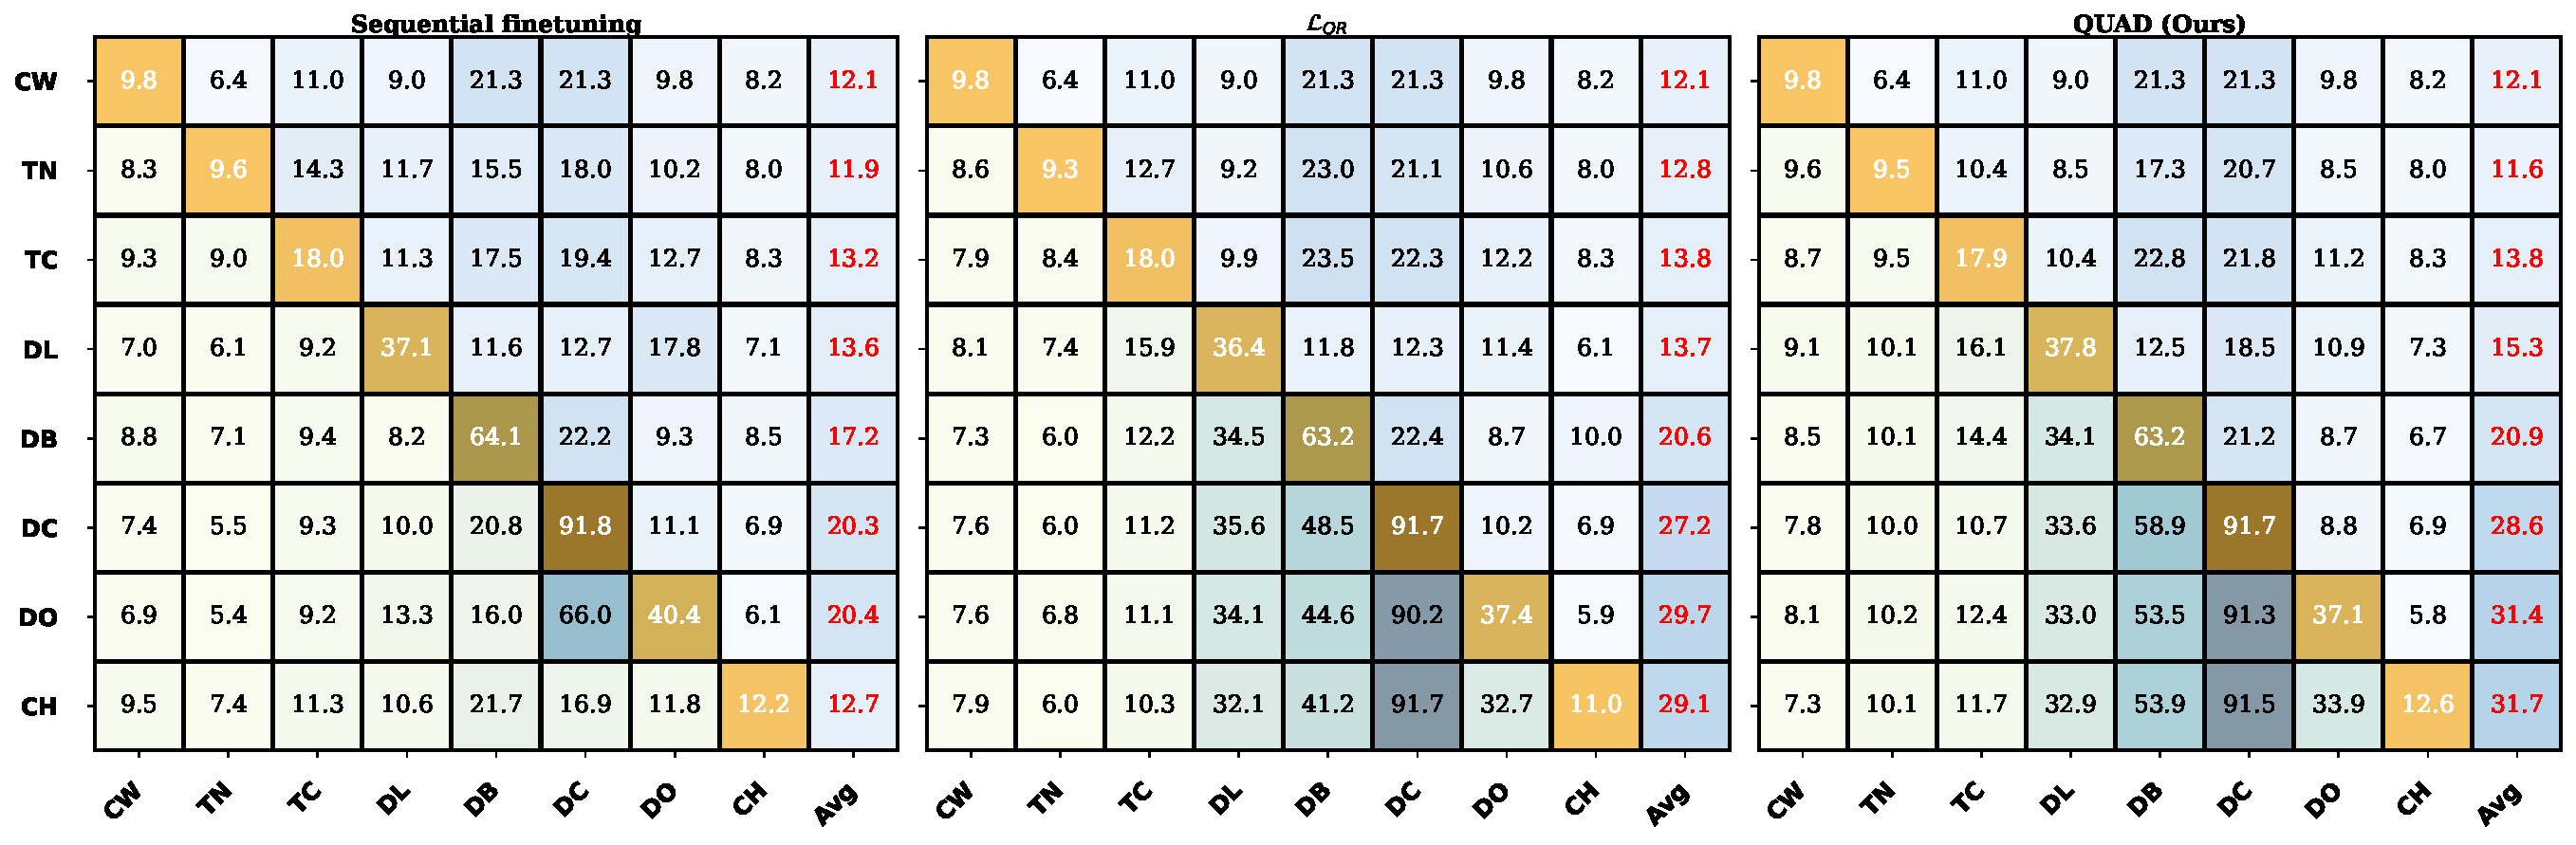
\includegraphics[width=\textwidth]{Figures/matrix_plots_nextqa.pdf}
    \caption{Comparison of feature distillation methods on \textbf{NExT-QA}. Each matrix shows the performance of a model trained on tasks (rows) and evaluated on tasks (columns). The diagonal (highlighted in {\color{orange}{orange}}) represents in-domain performance, while off-diagonal elements show cross-domain generalization. Higher values (darker colors) indicate better performance.}
    \label{fig:cross_task_generalization_nextqa}
\end{figure*}

\section{Continual Learning Methods}
\label{explain_methods}
We assess and benchmark five prominent continual learning methods, encompassing two regularization techniques (EWC \citep{kirkpatrick2017overcoming}, MAS \citep{mas2018}) and three rehearsal-based methods (ER \citep{chaudhry2019tinyepisodicmemoriescontinual}, DER \citep{Chaudhry2019er}, VS \citep{Wan_2022_CVPR}, and VQACL\citep{zhang2023vqacl}). To ensure a consistent evaluation, all methods are implemented using their official codebases and integrated into the same transformer backbone as described in Section 5.1. 

\textbf{EWC} \citep{kirkpatrick2017overcoming} is a regularization method designed to preserve knowledge of prior tasks by selectively reducing updates on critical parameters. This is achieved by leveraging the Fisher Information Matrix, which quantifies the importance of parameters and incorporates an auxiliary L2 loss between significant parameters from old and new tasks.

\textbf{MAS} \citep{mas2018} similarly applies regularization, aiming to prevent significant changes to parameters vital for previous tasks by introducing an L2 loss. In contrast to EWC, MAS measures the sensitivity of the output with respect to parameter perturbations to estimate parameter importance.

\textbf{ER} \citep{chaudhry2019tinyepisodicmemoriescontinual} is a rehearsal method that utilizes a fixed-size memory buffer, where visited examples are stored and randomly sampled for retraining. In line with our approach, the memory size for ER is fixed at 5,000 for VQA v2 and 500 for NExT-QA. Given its simplicity and effectiveness, ER serves as the baseline for our proposed method.

\textbf{DER} \citep{Chaudhry2019er} is another rehearsal technique that employs reservoir sampling to manage memory, ensuring every visited sample has an equal chance of being stored. DER also incorporates a dark knowledge distillation strategy, which aims to align the network’s outputs with logits recorded during training, thus encouraging consistency in responses to prior examples. In our experiments, DER also utilizes memory sizes of 5,000 for VQA v2 and 500 for NExT-QA.

\textbf{VS} \citep{Wan_2022_CVPR} is a rehearsal-based method that emphasizes feature consistency between current and past data. To address forgetting, VS introduces two losses: a neighbor-session model coherence loss and an inter-session data coherence loss. For more details, we refer readers to \citet{Wan_2022_CVPR}. The memory size for VS is similarly set to 5,000 for VQA v2 and 500 for NExT-QA.

\textbf{VQACL} \citep{zhang2023vqacl} represents a rehearsal-based approach, incorporating a prototype module to learn both task-specific and invariant features, facilitating robust and generalizable representations for VQA tasks.
